%\clearpage
\section{Risultati}
\label{sec:risultati}
I programmi sono stati eseguiti mediante il seguente comando:
\begin{quotation}
\script{bash eserc\_lab.sh -a 20}
\end{quotation}
che esegue l'intero processo, generando 20 problemi simili per ogni incremento della densità dei nodi, pari a $10$, per le istanze \emph{casuali} e \emph{cluster}; mentre vengono generati solamente 20 problemi con istanze \emph{circolari} in quanto non è presente casualità nella loro generazione.

In totale sono quindi state generate $1020$ istanze, $200$ di tipo casuale, $800$ di tipo cluster e $20$ di tipo circolare.

I grafici riportano sull'asse delle ascisse il numero di nodi del problema, mentre sull'asse delle ordinate il tempo in secondi che è servito per trovare la soluzione, da notare che si è scelto di rappresentare il tempo in scala logaritmica.

I punti di interesse sono quelli identificati dal simbolo presente nella legenda di ogni grafico e rappresentano la media dei risultati ottenuti per le istanze simili, mentre le linee verticali indicano la variabilità nei risultati individuata tramite la deviazione standard.

\subsection{\acronimo{cplex}}
\begin{figure}[htb]
	\centering
	\begin{subfigure}[b]{.45\textwidth}
		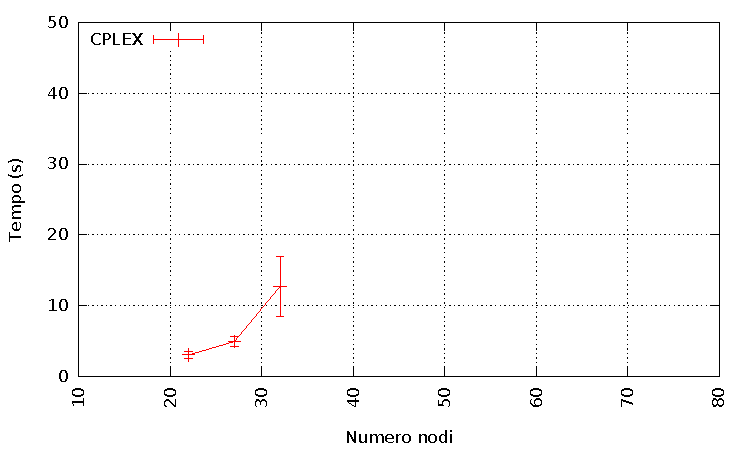
\includegraphics[width=\textwidth]{immagini/cplex_casuali.pdf}
		\caption{Istanze casuali}
		\label{fig:casuali cplex}
	\end{subfigure}
	\quad
	\begin{subfigure}[b]{.45\textwidth}
		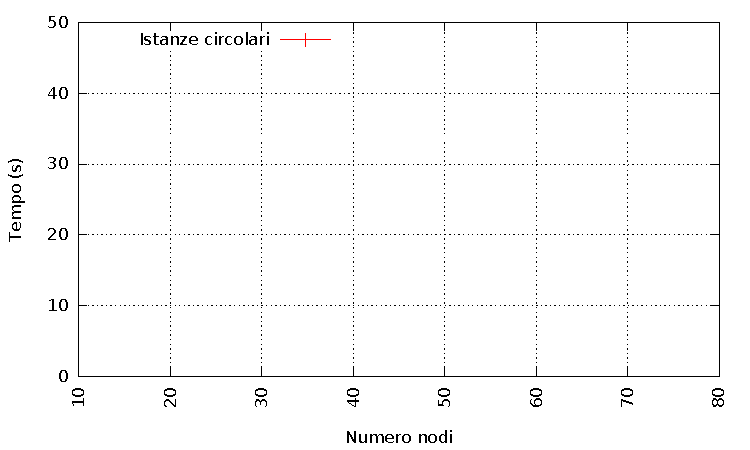
\includegraphics[width=\textwidth]{immagini/cplex_circolari.pdf}
		\caption{Istanze circolari}
		\label{fig:circolari cplex}
	\end{subfigure}
	\caption{Istanza casuali e circolari - \script{cplex}}
	\label{fig:casuali circolari cplex}
\end{figure}

In figura \ref{fig:casuali cplex} vediamo i risultati per le istanze casuali, esse seguono un andamento abbastanza regolare con il crescere del numero dei nodi: per istanze piccole il tempo di risoluzione è abbastanza rapido, ma sale molto velocemente, fino a oltre $200s$, con l'aumentare dei nodi.

Per quanto riguarda le istanze circolari, vediamo in figura \ref{fig:circolari cplex} che i tempi sono molto più bassi, rispetto alle istanze casuali, con un alto numero di nodi: questo è dovuto alla semplicità intrinseca di queste istanze che sono quindi più facili da risolvere.
Da notare come l'andamento del grafico non sia molto lineare: questo fatto probabilmente è dovuto al carico del processore al momento dell'esecuzione del test, che può non essere stato costante durante il periodo di prova.

Tutti i tempi ottenuti sono visibili nella tabella \ref{tab:casuali} per le istanze casuali e in tabella \ref{tab:circolari} per quelle circolari.

\begin{table}[htb]
	\centering
	\caption{Tempi istanze casuali - \script{cplex}}
	\label{tab:casuali}
	\begin{tabular}{cS[table-format=3.4]S[table-format=2.4]}
	\toprule
	\multirow{2}*{Numero nodi} 	& {Media} 	& {Deviazione standard} \\
								& {(s)}		& {(s)} \\
	\midrule
	11							& 0.3365	& 0.1538 \\
	16							& 0.9221	& 0.5562 \\
	20							& 1.6315	& 0.8956 \\
	25							& 3.5753	& 1.0769 \\
	29							& 7.7360	& 3.1880 \\
	34							& 24.0990	& 13.9010 \\
	38							& 44.4045	& 20.1608 \\
	43							& 94.7954	& 14.3456 \\
	47							& 133.3660	& 33.3648 \\
	52							& 252.7102	& 61.0620 \\
	\bottomrule
	\end{tabular}
\end{table}

\begin{table}[htb]
	\centering
	\caption{Tempi istanze circolari - \script{cplex}}
	\label{tab:circolari}
	\begin{tabular}{cS[table-format=1.4]cS[table-format=1.4]}
	\toprule
	\multirow{2}*{Numero nodi} 	& {Media} 	& \multirow{2}*{Numero nodi} 	& {Media} \\
								& {(s)}		& 								& {(s)} \\
	\midrule
	8	& 0.0861 &	48	& 1.4214 \\
	12	& 0.1108 &	52	& 2.6400 \\
	16	& 0.0707 &	56	& 2.3625 \\
	20	& 0.2480 &	60	& 2.1849 \\
	24	& 0.3751 &	64	& 2.3507 \\
	28	& 0.2500 &	68	& 3.4395 \\
	32	& 0.5208 &	72	& 3.4457 \\
	36	& 0.8440 &	76	& 3.2478 \\
	40	& 1.4215 &	80	& 5.0695 \\
	44	& 1.2282 &	84	& 6.0360 \\
	\bottomrule
	\end{tabular}
\end{table}

\begin{figure}[htb]
	\centering
	\begin{subfigure}[b]{.45\textwidth}
		\includegraphics[width=\textwidth]{immagini/cplex_cluster_1.pdf}
		\caption{Istanze 1 cluster}
	\end{subfigure}
	\quad
	\begin{subfigure}[b]{.45\textwidth}
		\includegraphics[width=\textwidth]{immagini/cplex_cluster_2.pdf}
		\caption{Istanze 2 cluster}
	\end{subfigure}
	\\
	\begin{subfigure}[b]{.45\textwidth}
		\includegraphics[width=\textwidth]{immagini/cplex_cluster_3.pdf}
		\caption{Istanze 3 cluster}
	\end{subfigure}
	\quad
	\begin{subfigure}[b]{.45\textwidth}
		\includegraphics[width=\textwidth]{immagini/cplex_cluster_4.pdf}
		\caption{Istanze 4 cluster}
	\end{subfigure}
	\caption{Istanze cluster - \script{cplex}}
	\label{fig:cluster cplex}
\end{figure}

In figura \ref{fig:cluster cplex} sono riportati i grafici riguardanti le istanze cluster: si può notare come abbiano tutti un andamento simile con tempi di risoluzione comparabili eccezion fatta per le istanze con $2$ nodi a $1$ cluster che hanno richiesto un tempo molto inferiore.

L'unico aspetto da sottolineare è la deviazione standard molto alta sulle istanze con $28$ nodi a $2$ cluster che è dovuta probabilmente ad un'istanza particolare che ha richiesto un tempo di risoluzione molto superiore alle altre.

\begin{figure}[htb]
	\centering
	\includegraphics[width=\textwidth]{immagini/cplex_all.pdf}
	\caption{Istanze casuali, cluster e circolari - \script{cplex}}
	\label{fig:all cplex}
\end{figure}

Ho deciso di riportare un grafico completo di tutti i risultati ottenuti, questo è visibile in figura \ref{fig:all cplex}.
È possibile vedere come con ogni tipologia di istanza, tranne quelle circolari, a parità di numero di nodi e quindi di complessità del problema, l'andamento del programma è simile.

È presente solo un leggero aumento nei tempi per quanto riguarda le istanze a 2 cluster: esse infatti sono costruite utilizzando due quarti opposti della griglia, creando quindi maggiori difficoltà nella risoluzione.

\subsection{Tabu Search}